\chapter{Artificial neural networks} % (fold)
\label{cha:artificial_neural_networks}
% What is it
Artificial neural networks are models that can approximate discrete-valued, real-valued and vector-valued functions.
They are composed of interconnected units that can activate others using connections of varying strength.
%citation?
Artificial neural networks are loosely inspired by biological neural networks, where these units are called neurons, which are connected by axons.\\
The higher the strength, also called weight, of connections between units, the more influence the unit has on the next one. These strengths can be manually defined. However, thanks to a method called backpropagation, weights can be learned systematically.
The combination of artificial neural networks and backpropagation led to successful applications, for example to recognize handwritten characters \citep{journals/neco/LeCunBDHHHJ89}, for face recognition \citep{cottrell1990extracting} and to recognize spoken words \citep{journals/nn/LangWH90}.
However, early applications also include reinforcement learning, for example to learn to balance a pendulum \citep{anderson:ieeecsm89} or to play the game \textit{Backgammon} \citep{Tesauro:92}.

\section{Basics} % (fold)
\label{sec:basics}
As said, artificial neural networks are made up of units. These units can be divided into layers, where the values of each layer are propagated to the next layer depending on connections with weights. These weights define the model.
Input units receive information that is available externally and provide information to other units. Output units are the opposite and receive information from the network itself and provide information externally. Hidden units both receive information from and provide information to units inside the network.\\
A simple artificial neural network is visualized in Figure~\ref{fig:ann}.\\
\begin{figure}[htb]
    \centering
    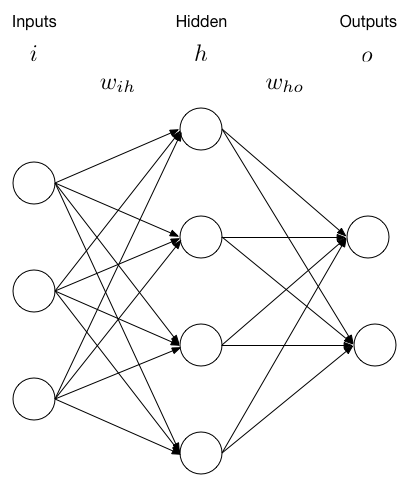
\includegraphics[width=.7\linewidth]{images/ann.png}
    \caption[An artificial neural network]{An artificial neural network with 3 input units, 4 hidden units and 2 output units. $w_{ih}$ and $w_{ho}$ are the weights for connections between respectively the input units and hidden units and between the hidden units and output units.}
    \label{fig:ann}
\end{figure}
As a non-input unit gets weighted activations from multiple units, these need to be combined to determine if the unit can be activated or not. This is done by applying a linear or non-linear function, called an activation function, to the weighted sum.
% section basics (end)

\section{Activation functions} % (fold)
\label{sec:activation_functions}
Formally, an activation function $\phi$ will compute for unit $j$ with inputs from layer $x$:
\begin{equation}
    o = \phi\big(\sum_i^n w_{ij} x_i\big)
\end{equation}
Or in vector format:
\begin{equation}
    o = \phi(\overrightarrow{w} \cdot \overrightarrow{x})
\end{equation}
From hereon we will denote the weighted sum as $z \equiv \sum_i^n w_{ij} x_i \equiv \overrightarrow{w} \cdot \overrightarrow{x}$.\\

\subsection{Perceptron} % (fold)
\label{ssub:perceptron}
A perceptron unit, defined by \cite{Rosenblatt58}, gives as output either $-1$ or $+1$ depending on the linear combination of the input and the weights:
\begin{equation}
o(\overrightarrow{x}) = \begin{cases}
+1 & \text{if $ \overrightarrow{w} \cdot \overrightarrow{x} > 0$}\\
-1 & \text{otherwise}
\end{cases}
\end{equation}
It can be seen as a hyperplane where the output is $-1$ or $+1$ depending on which side the input lies.
Using $-1$ as \texttt{false} and $+1$ as \texttt{true}, it is also possible to represent boolean functions such as \textit{AND}, \textit{OR}, \textit{NAND} and \textit{NOR}. However, some boolean functions, such as \textit{XOR} cannot be represented by a single perceptron \citep{ML}.

A schematic using the perceptron unit is shown in Figure~\ref{fig:perceptron}.\\
\begin{figure}[htb]
    \centering
    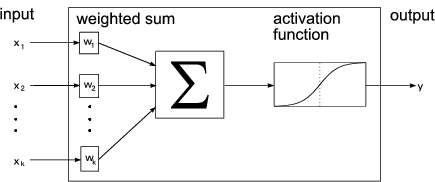
\includegraphics[width=\linewidth]{images/activation_functions/perceptron.png}
    \caption[The perceptron unit]{The perceptron unit. Source: \cite{Demant2013}.}
    \label{fig:perceptron}
\end{figure}
% subsection perceptron (end)

\subsection{Sigmoid} % (fold)
\label{ssub:sigmoid}
A disadvantage of the perceptron unit is that it is not differentiable in the whole domain (specifically at $x=0$). Why this is a problem will become clear in Section~\ref{sec:gradient_descent_and_backpropagation}.\\
To solve this problem, a sigmoid function can be used. A sigmoid function is a differentiable function that is monotonically increasing and approaches an asymptote for $x \to \pm\infty$ \citep{series/lncs/LeCunBOM12}. As a result, these can still separate the input space in 2 parts.\\
In the artificial neural networks domain, the \textit{sigmoid function} generally refers to a variation of the logistic function and is denoted by $\sigma(x)$. Its formula is:
\begin{align}
    \begin{split}
        f(z) &= \sigma(z)\\
        &= \frac{1}{1+e^{-z}}
    \end{split}
\end{align}
The behavior of this function is visualized in Figure~\ref{fig:sigmoid}.
\begin{figure}[htb]
    \centering
    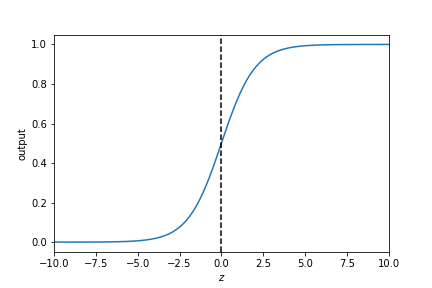
\includegraphics[width=.8\linewidth]{images/activation_functions/sigmoid.png}
    \caption[The sigmoid function]{The sigmoid function.}
    \label{fig:sigmoid}
\end{figure}
% subsection sigmoid (end)

\subsection{Hyperbolic tangent} % (fold)
\label{ssub:hyperbolic_tangent}
Another popular function and another kind of sigmoid function is the hyperbolic tangent function, also called \textit{tanh}. While the output of the sigmoid function ranges between $0$ and $+1$, here the output ranges between $-1$ and $+1$, just like the range (and the only possible values) of the perceptron.
The formula of the hyperbolic tangent function, which can also be written in terms of the sigmoid function, is:
\begin{align}
    \begin{split}
        f(z) &= tanh(z)\\
        &= 2\sigma(2z) - 1\\
        &= \frac{e^{\frac{z}{2}} - e^{-\frac{z}{2}}}{e^{\frac{z}{2}} + e^{-\frac{z}{2}}}
    \end{split}
\end{align}
This function is visualized in Figure~\ref{fig:tanh}.
\begin{figure}[htb]
    \centering
    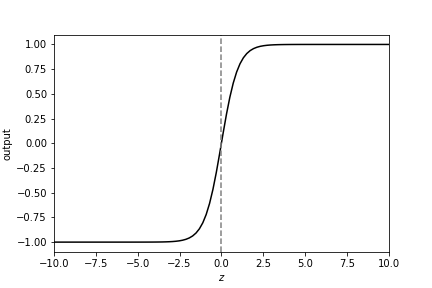
\includegraphics[width=.8\linewidth]{images/activation_functions/tanh.png}
    \caption{Hyperbolic tangent function.}
    \label{fig:tanh}
\end{figure}
% subsection hyperbolic_tangent (end)

\subsection{Rectified Linear Unit} % (fold)
\label{ssub:rectified_linear_unit}
A rectified linear unit, also called a ReLU, is another popular and more recent activation function. It was first defined by \cite{conf/icml/NairH10}. The output is the identity function if $z \ge 0$ and $0$ otherwise:
\begin{equation}
    f(z) = \begin{cases}
        z & \text{if $z \ge 0$}\\
        0 & \text{otherwise}
        \end{cases}
\end{equation}
As can be seen, this function requires less computations than the sigmoid and hyperbolic tangent function. However, the derivative for $z<0$ is always $0$. Why this can be a problem is also explained in Section~\ref{sec:gradient_descent_and_backpropagation}.\\
The ReLU function is shown in Figure~\ref{fig:relu}.
\begin{figure}[htb]
    \centering
    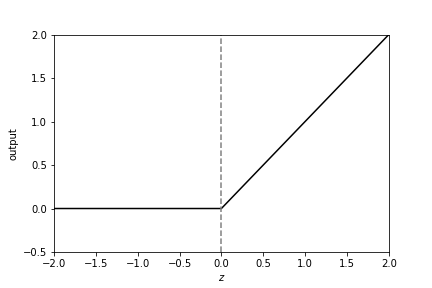
\includegraphics[width=.8\linewidth]{images/activation_functions/relu.png}
    \caption[Rectified Linear Unit function]{Rectified Linear Unit function.}
    \label{fig:relu}
\end{figure}

To solve the problem of the derivative being zero at $z<0$, the Leaky ReLU was invented \citep{maas2013rectifier}. Here, instead of the output being zero for $z<0$, the output has a small slope, defined by a constant $\alpha$:
\begin{equation}
    f(z) = \begin{cases}
        z & \text{if $z \ge 0$}\\
        \alpha z & \text{otherwise}
        \end{cases}
\end{equation}
As can be seen, the derivative of this function is always non-zero.\\
An example of a Leaky ReLU is shown in Figure~\ref{fig:lrelu}.\\
\begin{figure}[htb]
    \centering
    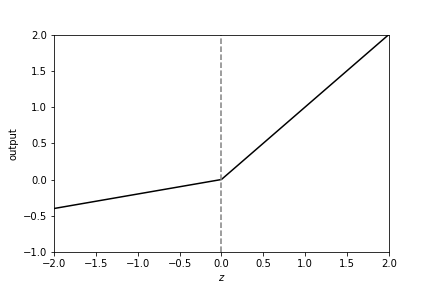
\includegraphics[width=.8\linewidth]{images/activation_functions/lrelu.png}
    \caption[Leaky ReLU function]{Leaky ReLU function with $\alpha = 0.2$.}
    \label{fig:lrelu}
\end{figure}
% subsection rectified_linear_unit (end)
% section activation_functions (end)

A variation of a Leaky ReLU, called Parametric Rectified Unit, also has a small slope for $x<0$, but with an $\alpha$ that can be learned \citep{journals/corr/HeZR015}. Other variants use a random slope for values below zero \citep{journals/corr/XuWCL15}, add noise a ReLU \citep{conf/icml/NairH10} or use an exponential function for values below zero \citep{journals/corr/ClevertUH15}:
\begin{equation}
    f(z) = \begin{cases}
        z & \text{if $z \ge 0$}\\
        \alpha (e^z-1) & \text{otherwise}
        \end{cases}
\end{equation}

\todo{Add softmax (used in my network)}


\section{Gradient descent and backpropagation} % (fold)
\label{sec:gradient_descent_and_backpropagation}
%Also something about linearly separable?
%Why no algebraic solution?
If we choose the weights of our network correctly, we might succeed in approximating a function.
However, it is not always possible to separate the input space and have the right with our artificial neural network.
In that case, we might want the best solution, e.g. one that has the least amount of errors in producing outputs w.r.t. the correct outputs, also called the target outputs. Furthermore, choosing the weights manually can be a tedious process.\\
For these reasons, we use an algorithm called called backpropagation, which uses a variation of gradient descent. We will first discuss gradient descent as this provides the basis of the backpropagation algorithm.

\subsection{Gradient descent} % (fold)
\label{ssub:gradient_descent}
In gradient descent, we search in the weight vector space, also called hypothesis space, to find weights that can approximate a function as best as possible. A tuple containing the input and output of the target function is called a training example.

To be able to update weights, we first need to know how wrong our outputs were relative to those of our training examples.
This is called the training error and depends on the learning algorithm (in our case an artificial neural network), its parameters and the training examples. However, here we assume that the learning algorithm and the training examples are fixed while learning.
A common measure for the training error, the mean squared error (MSE), is defined as:
\begin{equation}
    E(\overrightarrow{w}) \equiv \frac{1}{N} \sum_{i=0}^N (y_i - f(x_i;\overrightarrow{w}))^2
\end{equation}
Where $N$ is the number of training examples, $x_i$ is the input of a training example, $y_i$ is the target output of the training example and $f$ is our learning algorithm, which depends on the weight vector $\overrightarrow{w}$.\\

Because we now know how the training error and the weight vector are related, we can compute the derivative of the training error $E$ with respect to each component of $\overrightarrow{w}$. This called the gradient and is denoted as $\nabla E(\overrightarrow{w})$:
\begin{equation}
    \nabla E(\overrightarrow{w}) \equiv \left [ \frac{\partial E}{\partial w_0}, \frac{\partial E}{\partial w_1}, \dots, \frac{\partial E}{\partial w_n} \right ]
\end{equation}
Where $n$ is the number of components in $\overrightarrow{w}$. Note that $\nabla E(\overrightarrow{w})$ is also a vector. It defines how to change the weight components in order to get the steepest increase in the training error $E$. Thus, if we negate the gradient, we get the steepest decrease in $E$. We can then update the weight vector as such:
\begin{equation}
    \overrightarrow{w} \gets \overrightarrow{w} - \eta \nabla E(\overrightarrow{w})
\end{equation}
Where $\eta$ is a positive value called the learning rate, which influences how big the changes to the weight vector are.\\

The goal is to set the weights to such values so that the error is minimized. This is called a global minimum. No other combinations of weight values can lead to a lower error than those of the global minima.\\
However, it is possible that, given a combination of weight values, any change in those values does not influence the error, in which case the gradient for every weight component is $0$. Thus, with the current algorithm, there is no incentive to change the weights. This is called a local minimum. Although the algorithm cannot "see" immediate improvements, it is possible that another combination of weight values leads to a lower error. This is analogous to being in a valley in the mountains, where the valley after a mountain (and thus not visible) may lie lower. This is also visualized in Figure~\ref{fig:error_surface}.\\
\begin{figure}[htb]
    \centering
    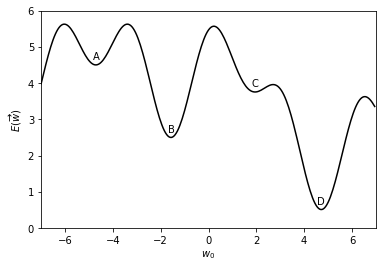
\includegraphics[width=\linewidth]{images/error_surface.png}
    \caption[An example of an error surface]{An example of an error surface using only one weight $w_0$. \textit{A}, \textit{B} and \textit{C} are local minima, while \textit{D} is the global minimum.}
    \label{fig:error_surface}
\end{figure}

For artificial neural networks without a hidden layer, such as a single perceptron unit, that use the MSE when updating weights, every local minimum is also a global minimum. However, when using hidden layers, this might not always be the case.\\
These local minima might seem like a problem for artificial neural networks, but in practice they rarely are, according to theoretical and empirical results \citep{choromanska2015loss}.
Instead, there are more saddle points. Here, the gradient is zero and the error goes up when some weights are changed and goes down for others. Generally a lot of such points are present, but they all have the same value for the objective function (i.e. the error function).\\

A small value of $\eta$ leads to slow convergence, while a high value can cause the algorithm to overstep a local minimum. Because of this, the some algorithms gradually decrease the learning rate as the number of weight updates grows.\\
For a single weight component, we get:
\begin{equation}
    \label{eq:weightcomponentupdate}
    w_i \gets w_i - \eta \frac{\delta E}{\delta w_i}
\end{equation}

Of course, in order to update the weights, we first need to calculate the derivate of $E$ w.r.t. each component $w_i$. As an example, we show the derivative when using a simple linear unit, which defined as:
\begin{equation}
    f(\overrightarrow{x};\overrightarrow{w}) = \overrightarrow{x} \cdot \overrightarrow{w}
\end{equation}
We then get the following derivation:
\begin{align}
    \label{eq:gradderiv}
    \begin{split}
        \frac{\delta E}{\delta w_i} &= \frac{\delta}{\delta w_i} \frac{1}{N} \sum_{j=0}^N (y_j - o_j)^2\\
        &= \frac{1}{N} \sum_{j=0}^N \frac{\delta}{\delta w_i} (y_j - o_j)^2\\
        &= \frac{1}{N} \sum_{j=0}^N 2 (y_j - o_j) \frac{\delta}{\delta w_i} (y_j - o_j)\\
        &= \frac{2}{N} \sum_{j=0}^N (y_j - o_j) \frac{\delta}{\delta w_i} (y_i - \overrightarrow{x_i} \cdot \overrightarrow{w})\\
        &= \frac{2}{N} \sum_{j=0}^N (y_j - o_j)(-x_{ij})
    \end{split}
\end{align}
Where $x_{ij}$ is the $i$'th input component of training example $j$ and $o_j \equiv f(x_j; \overrightarrow{w})$. Instead of just using a linear unit, the function $f$ can of course be more complex and use for example on of the activation functions from Section~\ref{sec:activation_functions}. However, we can now see that we cannot use the perceptron because it is not differentiable.\\

Using the resulting formula of Equation~\ref{eq:gradderiv} along with Equation~\ref{eq:weightcomponentupdate}, we can also define how to update each component of the weight vector:
\begin{equation}
    w_i \gets w_i + \eta \frac{2}{N} \sum_{j=0}^N (y_j - o_j)x_{ij}
\end{equation}
As we can see, for each weight vector, we need to apply the model to the input of each training example. For this reason, this version of gradient descent is also often called \textit{batch gradient descent}. Of course, the outputs only need to be computed once per weight vector update as they do not depend on which specific weight vector component that we are updating.\\

Still, each time using every training example for the weight vector update can lead to slow convergence to a local minimum. Furthermore, in case of multiple local minima in the error surface, it is possible that the gradient descent algorithm does not stop at the global minimum \citep{ML}.
% subsection gradient_descent (end)

\subsection{Stochastic gradient descent} % (fold)
\label{ssub:stochastic_gradient_descent}
A popular variation of batch gradient descent that tries to solve the previously mentioned issues is \textit{stochastic gradient descent}. Instead of summing using all training examples, we do a weight update using only one training example. To do this, we first use a different error function for each example $j$:
\begin{equation}
    E_j(\overrightarrow{w}) = (y_j - o_j)^2
\end{equation}
The update for a single weight vector component when using a linear unit is then:
\begin{equation}
    w_i \gets w_i + 2 \eta(y_j- o_j)x_{ij}
\end{equation}
The idea here is that these weight updates, when having iterated over all the training examples, will be a decent approximation relative to using our original error function. Note that the update using one training example affects the error of the next training example.\\

By making the learning rate small enough, usually smaller than with batch gradient descent, it is possible to approximate true gradient descent arbitrarily closely \citep{ML}.
It is also computationally cheaper because each time we only handle one training example.
Additionally, stochastic gradient descent can sometimes avoid being stuck in local minima because it uses various $\nabla E_j(\overrightarrow{w})$ instead of just $\nabla E(\overrightarrow{w})$ to move in the hypothesis space.
% subsection stochastic_gradient_descent (end)

\subsection{Backpropagation} % (fold)
\label{ssub:backpropagation}
The backpropagation algorithm uses gradient descent and can learn weights of a multilayer network with possibly multiple units in each layer \citep{rumelhart1986learning}.

We say that, for multilayer networks, $L>2$, with $L$ the number of layers in the network. This means that there are other (hidden) layers besides the input and output layer. Such a network was already depicted in Figure~\ref{fig:ann}.

As multiple output units are also possible, we need a new training error measure that sums over all of the output units of the network:
\begin{equation}
    E(\overrightarrow{w}) \equiv \frac{1}{N} \sum_{i=0}^N \sum_{k \in outputs} (y_{ki} - o_{ki})^2
\end{equation}
Where $outputs$ are the output units of the network and $y_{ki}$ and $o_{ki}$ is the value of the $k$'th output unit of respectively the $i$'th training example and network output.\\

The difference with calculating the weight changes in artificial neural networks with more than 2 layers is that, starting from the second non-input layer, the input to a unit comes, besides the weights, from other units of which the value itself is also calculated.
Thus, units in some layers can depend on units in multiple previous layers. This must also be taken into account when calculating the gradient for the output of those units.
To do this, we can use the chain rule for the gradient of a single weight component:
\begin{align}
    \frac{\partial E_d}{\partial w_{ji}} &= \frac{\partial E_d}{\partial net_j} \frac{\partial net_j}{\partial w_{ji}}\\
    &= \frac{\partial E_d}{\partial net_j} x_{ji}
\end{align}
Where $E_d$ is the error for a training example $d$, $x_{ji}$ is the $i$'th input to unit $j$, $w_{ji}$ is the weight associated with this input and $net_j = \sum_i w_{ji} x_{ji}$. The further derivation for all the weights of the network is described in \cite[Chapter~4]{ML}. For an artificial neural network with 1 hidden layer, we get the pseudo-code shown in Algorithm~\ref{algo:backpropagation}.\\
\begin{algorithm}[htb]
\DontPrintSemicolon
\KwIn{training\_examples, neural\_network, $\eta$}
\emph{// Assume a network with $n_{in}$ input units $n_{hidden}$ hidden units and $n_{out}$ output units.}\\
\emph{// Assume (randomly) instantiated weights.}\\
\Repeat{a termination condition is met}{
    \For{$(\overrightarrow{x},\overrightarrow{y})$ in training\_examples}{
        Propagate $\overrightarrow{x}$ through the network and receive values for all the output units: $o_u$ with $u$ an output unit of the network\\
        \For{each network output unit $k$}{
            Calculate its error term:\\
            $\delta_k \gets o_k(1-o_k)(y_k-o_k)$
        }
        \For{each hidden unit $h$}{
            Calculate its error term:\\
            $\delta_h \gets o_h(1-o_h) \sum_{k \in outputs} w_{kh}\delta_k$
        }
        \For{each network weight $w_{ji}$}{
            Do an update:\\
            $w_{ji} \gets w_{ji} + \Delta w_{ji}$\\
            where\\
            $\Delta w_{ji} = \eta \delta_j x_{ji}$ \label{algo:backpropagation:deltaweight}
        }
    }
}
\caption[Backpropagation]{Backpropagation algorithm. For simplicity, the squared error ($E_j(\overrightarrow{w}) = \frac{1}{2} (y_j - o_j)^2$ for training example $j$) was used. Source: \cite[Chapter~4]{ML}.}
\label{algo:backpropagation}
\end{algorithm}
% subsection backpropagation (end)

\subsection{Extensions and improvements} % (fold)
\label{ssub:extensions_and_improvements}
\subsubsection{Different loss functions} % (fold)
\label{ssub:loss_functions}
Besides just the difference between the output of the network and the expected output, additional penalties can be added to indirectly influence the values of the weights. This is generally done in order to prevent overfitting. Overfitting means that the performance of the algorithm on the data on which we trained (called \textit{training data}) is significantly better than the performance on held-out data on which we didn't train (called \textit{test data}). The algorithm captures too much details or noise in the training data. Using penalties, we can force the algorithm to focus on generalization rather than specialization.\\
Here, we typically use the term \emph{loss function} instead of an error function. This loss function can contain the error as we already described, along with other functions (typically also called loss functions).\\

A popular loss function is called the $L_1$ norm (also called Lasso) \citep{tibshirani1996regression}. For each weight $w$, we add the value $\lambda \vert w \vert$ to the loss. The $L_1$ norm is then defined as such:
\begin{equation}
    L_1(\overrightarrow{w}) = \lambda \sum_{i=1}^k \vert w_i \vert
\end{equation}
Where $k$ is the number of weights of the network and $\lambda$ is a parameter determining the regularization strength.
As the loss function, we then get:
\begin{equation}
    L(\overrightarrow{w}) = E(\overrightarrow{w}) + L_1(\overrightarrow{w})
\end{equation}
This norm has the property of leading to sparse weight vectors \citep{journals/ftml/BachJMO12}. This means that a lot of weights are zero or close to zero and the focus is on finding a subset of the must important units.
%neurons with L1 regularization end up using only a sparse subset of their most important inputs and become nearly invariant to the “noisy” inputs

Instead of using the absolute value, the $L_2$ norm sums over squared weights. It has the following form:
\begin{equation}
    L_2(\overrightarrow{w}) = \frac{1}{2} \sum_{i=1}^k w_i^2
\end{equation}
The fraction $\frac{1}{2}$ is often used such that the derivative is $\lambda w$ instead of $2 \lambda w$. The $L_2$ loss focuses more on penalizing high weights. It leads to diffusion of the weights and can indirectly force the network to use all the units of the network to form the correct output.
% notice that during gradient descent parameter update, using the L2 regularization ultimately means that every weight is decayed linearly: W += -lambda * W towards zero.

The $L_1$ and $L_2$ can also be combined, called \textit{elastic net regularization} \citep{hastie2012ElasticNet}:
\begin{align}
    L_E (\overrightarrow{w}) &= L_1(\overrightarrow{w}) + L_2(\overrightarrow{w})\\
    &= \sum_{i=1}^k \lambda_1 \vert w_i \vert + \lambda_2 w_i^2
\end{align}

% subsubsection loss_functions (end)

\subsubsection{Different weight updates} % (fold)
\label{ssub:different_weight_updates}
Here we discuss methods that, given an error function, update the weights in different ways.\\

One of the most common extensions to backpropagation is to add a fraction of the previous weight update to the new weight update. This extension is called \textit{momentum}.\\
To apply this, we change the equation on line~\ref{algo:backpropagation:deltaweight} of Algorithm \ref{algo:backpropagation} to the following:
\begin{equation}
    \Delta w_{ji}(t) = \eta \delta_j x_{ji} + \alpha \Delta w_{ji}(t-1)
\end{equation}
Where $\Delta w_{ji}(t)$ is a weight update executed at iteration $t$ and $\alpha$, with $0 \le \alpha < 1$, determines how much of the previous weight update we want to carry to the new one. When $\alpha = 0$, we get again the regular weight update.

Thanks to momentum, it is possible to get past regions where the gradient is zero and the weights would not change without momentum.
This is analogous to a ball rolling down a surface but keeps rolling a bit on a flat surface afterwards. In the real world, an object in motion will stay in motion, unless there is a force applied to it.
Here, that force is the gradient. It is also possible to get past small local minima and it can speed up learning when the gradient does not change. Again, this is analogous to a ball that goes downhill and keeps gaining speed.\\

The weight update of Root Mean Square Propagation (RMSProp) is quite different from stochastic gradient descent and only uses the sign of the gradient to update the weights \citep{Tieleman2012LectureMagnitude.}.
This allows us to escape from plateaus more quickly. Furthermore, the learning rate can be different for each weight.
For example, we can multiply the learning rate of a certain weight by a factor greater than one if its last 2 gradients agreed on the sign, and multiply the learning rate by a value less than $1$ otherwise.
This means that, when the gradients agree on the direction, we give them more influence. If they are not consistent and disagree in subsequent steps, we decrease the influence. We can also put a limit on the learning rate as to not let it grow to excessively low or high amounts.

However, by just using an adaptive learning rate, we can have the problem of weights themselves growing too high in unwanted situations. For example, when a gradient is for 9 subsequent steps a small positive amount (e.g. $0.1$) and once a large negative amount (e.g. $-0.9$), we don't want to change the weights a lot because they balance each other out.
Using the current algorithm however, the learning rate and as a result the weights would become too high because we only look at the signs and not the magnitude of the gradients.\\
Notice that, right now, we are dividing the gradient by its absolute value in order to just get $+1$ or $-1$ depending on the sign. It is however better to divide each weight by a moving average of the squared weight using the gradients of the past steps:
\begin{subequations}
\label{eq:rmsprop}
\begin{align}
MeanSquare(w, t) &= \gamma \cdot MeanSquare(w, t-1) + (1 - \gamma) \cdot \left (\frac{\partial E}{\partial w(t)} \right )^2 \\
w(t+1) &= w(t) - \frac{\alpha}{\sqrt{MeanSquare(w,t)}}\frac{\partial E}{\partial w(t)} \label{eq:rmsprop:weightupdate}
\end{align}
\end{subequations}
Where $w(t)$ is a weight at time step $t$, $\frac{\partial E}{\partial w(t)}$ is its gradient, $\alpha$ is the learning rate and $w_{t+1}$ is the new weight value. The past squared gradients are decayed by a value $\gamma$. Usually $\gamma=0.9$. It is also possible to add a small number $\epsilon$ (e.g. $\epsilon = 10^{-8}$) to the denominator in Equation~\ref{eq:rmsprop:weightupdate} to avoid division by zero.\\

Adaptive Moment Estimation (Adam) \citep{DBLP:journals/corr/KingmaB14} also uses an adaptive learning rate for each weight and an exponentially decaying average of previous squared gradients (also called the second moment). In addition, an exponentially decaying average of past gradients (also called the first moment) is also stored:
\begin{subequations}
\label{eq:adam:means}
\begin{align}
    Mean(w,t) &= \beta_1 \cdot Mean(w,t-1) + (1-\beta_1)\cdot \frac{\partial E}{\partial w(t)}\\
    MeanSquare(w, t) &= \gamma \cdot MeanSquare(w, t-1) + (1 - \gamma) \cdot \left (\frac{\partial E}{\partial w(t)} \right )^2
\end{align}
\end{subequations}
The authors of this method observed that the two previous equations are biased towards zero, which results in high weight updates. To alleviate this problem, the use bias-corrected values:
\begin{subequations}
\label{eq:adam:means:corrected}
\begin{align}
    \widehat{Mean(w,t)} &= \frac{Mean(w,t)}{1-\beta_1^t}\\
    \widehat{MeanSquare(w,t)} &= \frac{MeanSquare(w,t)}{1-\beta_2^t}
\end{align}
\end{subequations}
The weight update then becomes:
\begin{equation}
    w(t+1) = w(t) - \frac{\alpha}{\sqrt{MeanSquare(w,t)} + \epsilon} Mean(w,t)
\end{equation}
% subsubsection different_weight_updates (end)

\subsubsection{Dropout} % (fold)
\label{ssub:dropout}
Dropout is a way to prevent overfitting and is mostly applied to deep learning methods, which are explained in Chapter~\ref{cha:deep_learning}. It does so by randomly leaving out some visible or hidden units. As a result, all incoming and outgoing connections to these temporarily removed units are also removed and the algorithm can't rely on these connections. The simplest way of determining if a unit has to be removed is by removing it with a certain probability $p$, e.g. $p=0.5$. This value can also be determined by validation. As each unit can be present or not when using the network, for $n$ units there are $2^n$ possible networks.
By learning each time using a possibly different network, we have a way of combining multiple models where each model is trained only a few times and most weights are shared between other models. Dropout is only used when training. In the testing phase, no units are removed. Here, however, we multiply the outgoing weights of each unit by their probability $p$.
This is done to make sure that the \textit{expected} output for any hidden unit is the same as the actual output at test time.
% subsubsection dropout (end)

% subsection extensions_and_improvements (end)
% section gradient_descent_and_backpropagation (end)

% section artificial_neural_networks (end)
